\documentclass{article}
\usepackage[utf8]{inputenc}
\usepackage{hyperref}
\usepackage{graphicx}
\usepackage{float}
\usepackage{amsmath}

\providecommand{\tightlist}{%
  \setlength{\itemsep}{0pt}\setlength{\parskip}{0pt}}

\numberwithin{figure}{section}

\title{Carberry Pi Documentation}
\author{Ryan McHugh}
\date{April 2020}


\begin{document}

\maketitle


\begin{center}
\line(1,0){300}
\end{center}


\setcounter{secnumdepth}{2}

% // Logo

\textbf{Carberry Pi}

\begin{verbatim}

         11111111
        11   11   1
     111     11    1111
    111111111111111111111111
    1111001111111111110011111
      100001        100001
        00            00
\end{verbatim}

\hypertarget{outline-of-this-document}{%
\subsection{Outline of this Document}\label{outline-of-this-document}}

\begin{enumerate}
\def\labelenumi{\arabic{enumi}.}
\item
  \protect\hyperlink{introduction}{Introduction}
\item
  \protect\hyperlink{hardware}{Hardware}
\item
  \protect\hyperlink{software}{Carberry Pi Software}

  3.1 \protect\hyperlink{dashboard}{Dashboard}

  3.2 \protect\hyperlink{diagnostics}{Diagnostics}

  3.3 \protect\hyperlink{configuration}{Configuration}

  3.4 \protect\hyperlink{architecture}{Architecture}

\item
  \protect\hyperlink{connecting-the-pieces}{Connecting the Pieces}
\item
  \protect\hyperlink{getting-up-and-running}{Getting Up and Running}
\end{enumerate}

\hypertarget{introduction}{%
\section{Introduction}\label{introduction}}

\begin{itemize}
\tightlist
\item
  \emph{Carberry Pi} is an automotive application of a mini-computer in
  the car. As the quintessential project for my undergraduate studies,
  this concept provides a deep-dive into an area of future interest.
\end{itemize}

\hypertarget{hardware}{%
\section{Hardware}\label{hardware}}

Carberry Pi requires a few tools of the trade.\\

~~~~Namely:

\begin{itemize}
\item
  Raspberry Pi (this project uses a Raspberry Pi 3 model B)
\item
  Professional Grade OBDII Cable
\item
  Raspberry Pi Touchscreen
\item
 \href{https://thepihut.com/products/mini-rtc-module-for-raspberry-pi}{DS3231 RTC IC}
  (Real Time Clock)
\end{itemize}

\begin{figure}[H]
\centering
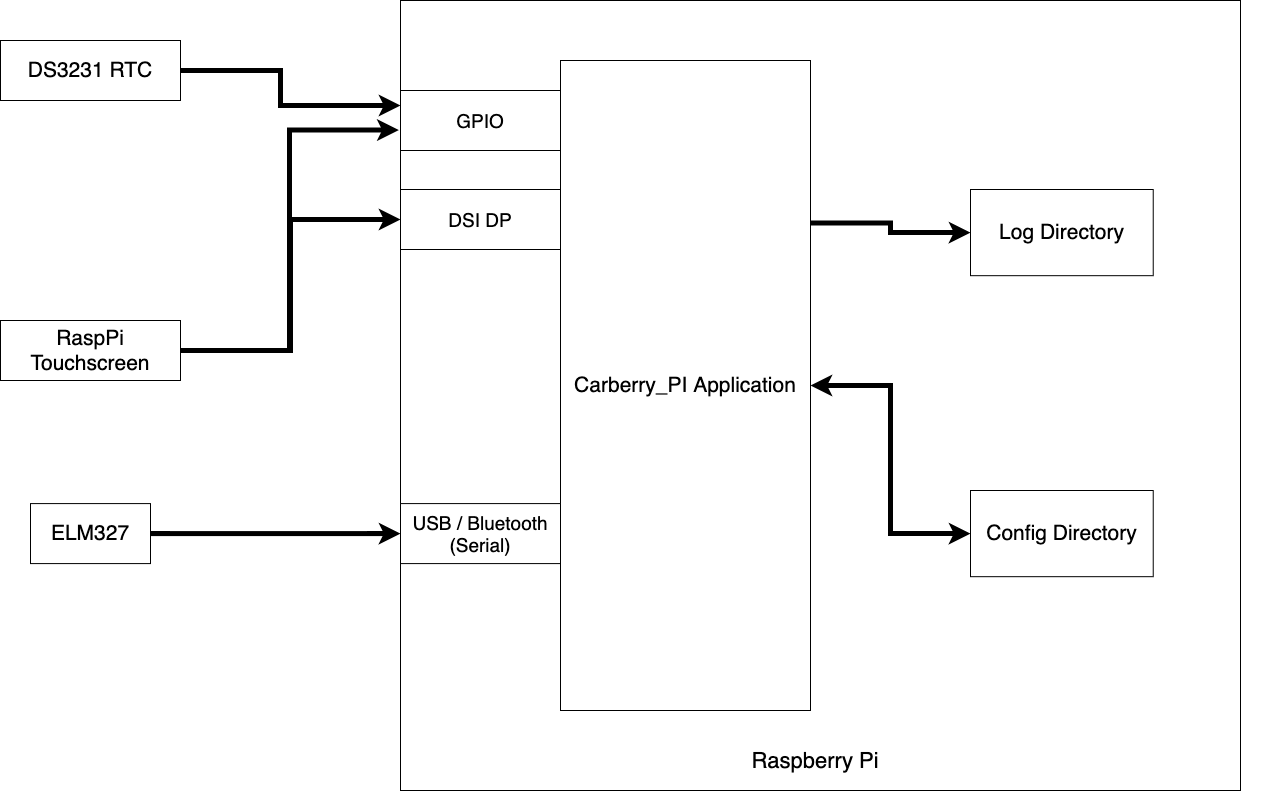
\includegraphics[width=1\columnwidth]{./diagrams/architecture/architecture_diagram.png}
\caption{Hardware Overview}
\end{figure}

\hypertarget{carberry-pi-software}{%
\section{Carberry Pi Software}\label{carberry-pi-software}}

\hypertarget{dashboard}{%
\subsubsection{Dashboard}\label{dashboard}}
Displays a speedometer, tachometer, and coolant temperature gauge.

\begin{figure}[H]
\centering
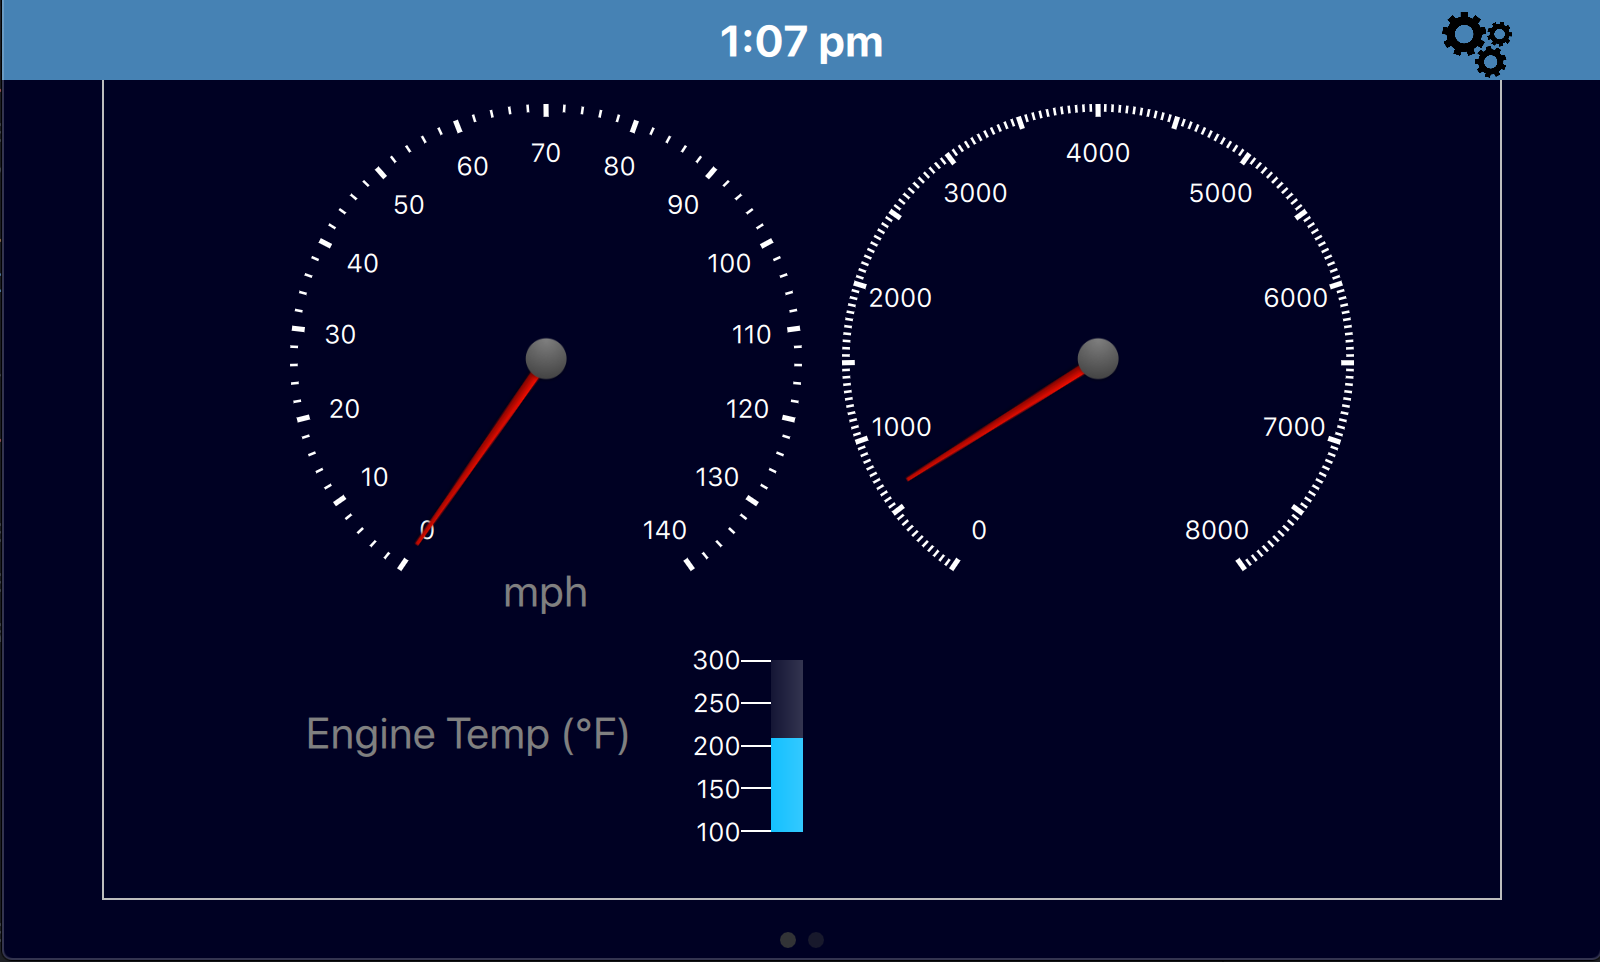
\includegraphics[width=0.7\columnwidth]{./resources/dash.png}
\caption{Dashboard}
\end{figure}

\hypertarget{diagnostics}{%
\subsubsection{Diagnostics}\label{diagnostics}}
Displays a list of all data points provided by the Car Computer.

\begin{figure}[H]
\centering
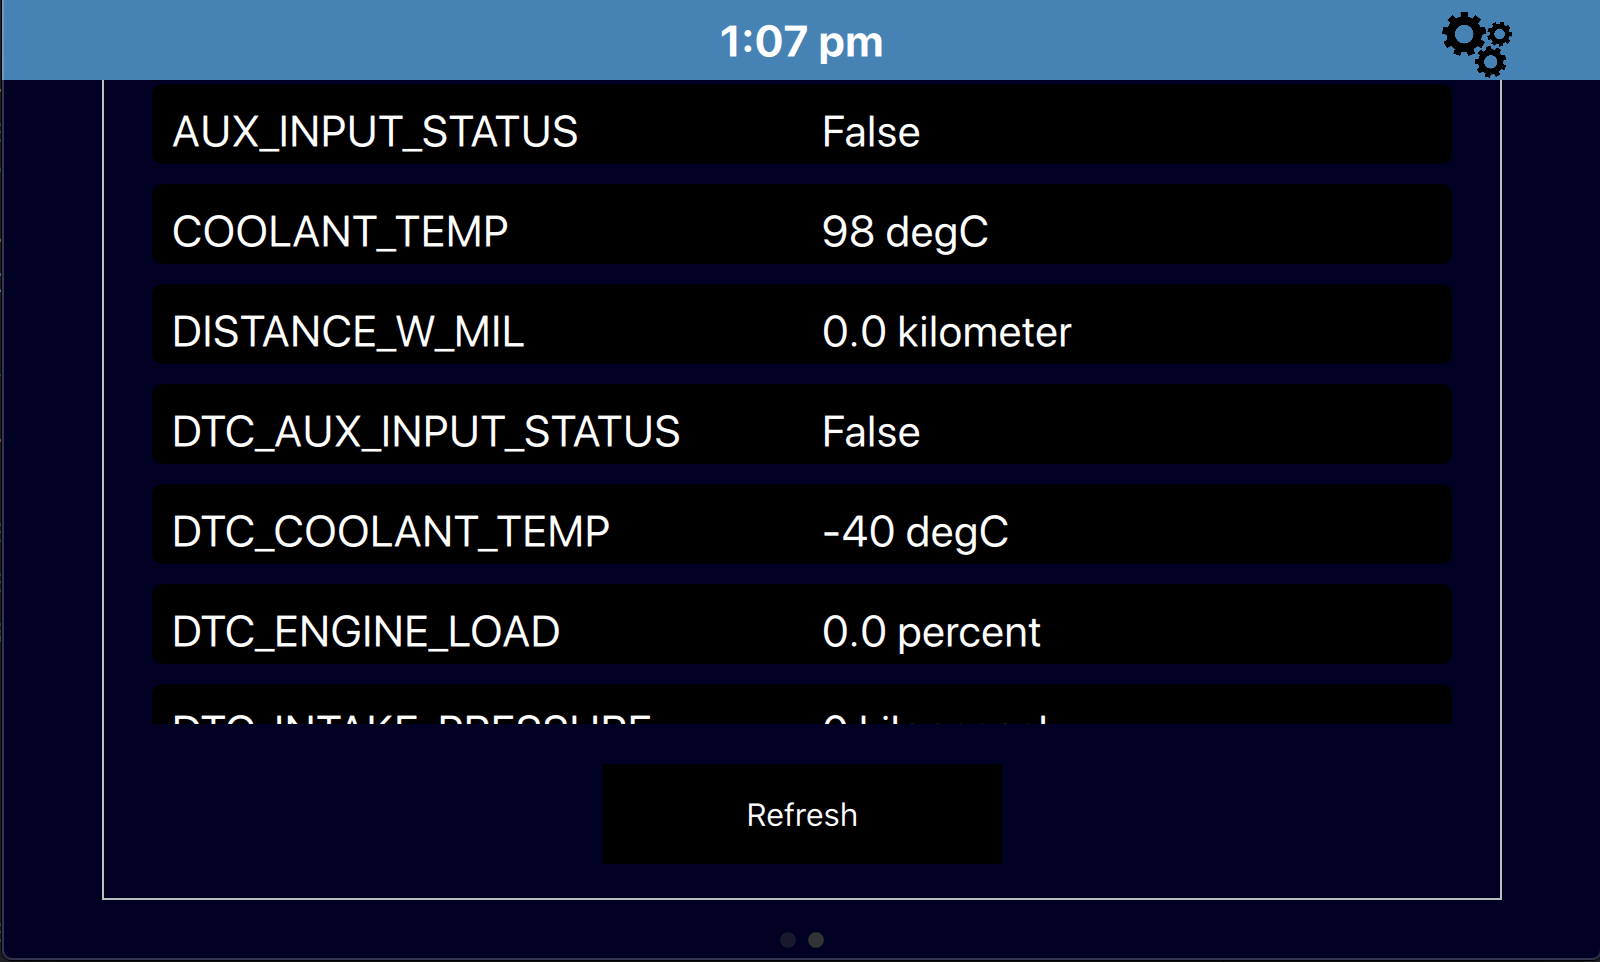
\includegraphics[width=0.7\columnwidth]{./resources/diagnostics.png}
\caption{Diagnostics}
\end{figure}

\hypertarget{configuration}{%
\subsubsection{Configuration}\label{configuration}}

\begin{figure}[H]
\centering
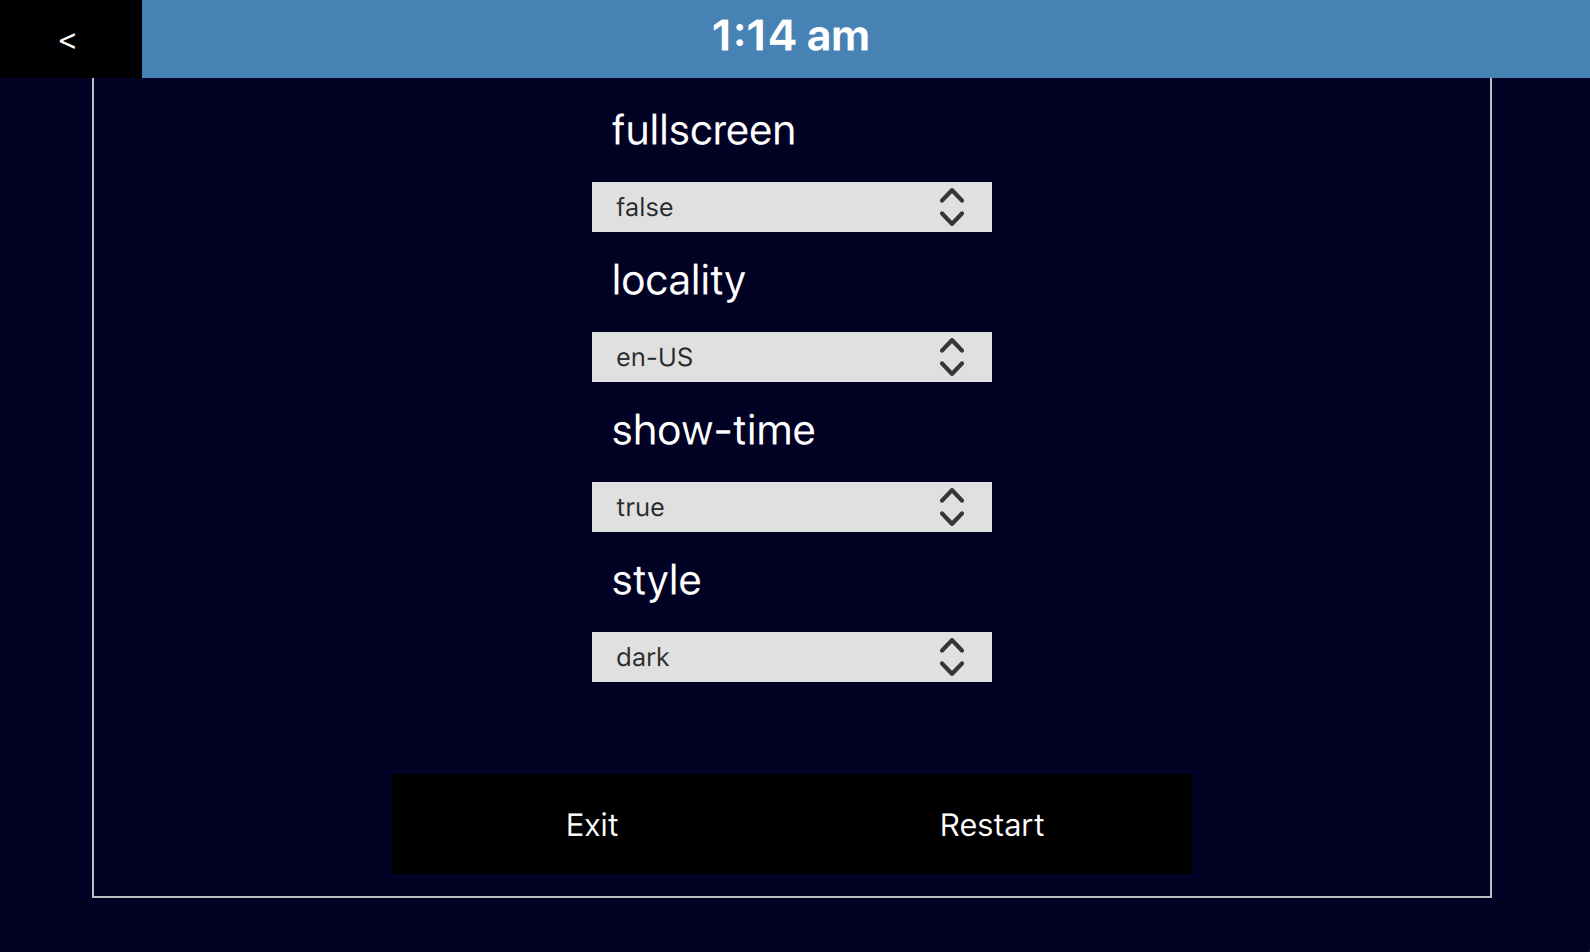
\includegraphics[width=0.7\columnwidth]{./resources/configuration.png}
\caption{Configuration}
\end{figure}

\subparagraph{Manage the settings of the application.}

\begin{itemize}
  \item
    locality: Region-based conversion of units (main dashboard only)
\end{itemize}
\begin{itemize}
  \item
    fullscreen: Toggle for fullscreen on startup (only works on
\end{itemize}
\begin{itemize}
  \item
    style: Manages the overall theme of the application (toggle between light and dark modes)
\end{itemize}
\begin{itemize}
  \item
    time: Show/Hide the time in the header bar
\end{itemize}

Application must be restarted for some preference changes to take effect.

\hypertarget{architecture}{%
\subsubsection{Architecture}\label{architecture}}

\hypertarget{toolkit}{%
\subparagraph{Toolkit}\label{Toolkit}}

\begin{itemize}
\item
  Backend: Python

  \begin{itemize}
  \tightlist
  \item
    Utilizes \href{https://python-obd.readthedocs.io/en/latest/}{python-obd} library for OBD information
  \end{itemize}
\item
  Frontend: PyQt (Qt-Quick) + QML \textbar{} Javascript
\end{itemize}

\hypertarget{interface-architecture}{%
\subparagraph{Interface Architecture}\label{interface-architecture}}

\begin{itemize}
\item
  Dynamic loading allows react.js style module instantiation and destruction

  \begin{itemize}
  \item
    Each component is loaded into a \emph{view} as a separate entity
  \item
    These components can then be pushed/popped onto or from the
    main\emph{stackview}
  \item
    A separate script (javascript) manages the creation/destruction of
    the \emph{back} button
  \end{itemize}
\item
  Time

  \begin{itemize}
  \item
    The time is based on the RTC (Real Time Clock) of the Raspberry Pi
    itself.
  \item
    As such, changing the locality has no effect on the time value.
  \end{itemize}
\end{itemize}

\subparagraph{Directory Structure \textbar{} File Enumeration}
\begin{itemize}
    \item \emph{documentation}: Stores the source files and compiled containers for this documentation\\
    \item \emph{src}: Contains the Project Source files

    \begin{itemize}
        \item \emph{items}: reusable \_custom\_ QML items
        \item \emph{js}: JavaScript scripts (primarily for object creation and destruction)
        \item \emph{log}: storage for log output \emph{(YYYY-MM-DD)}
        \item \emph{partials}: QML partials (snippets)
        \item \emph{resources}: assets \textbar{} icons
    \end{itemize}
\end{itemize}

\subparagraph{Runtime Overview}
{
  \emph{run.py} lasts the runtime of the program. It initializes the GUI through the pyqt application     engine. Then the front end initializes communication with \emph{run.qml}.  In the meantime, \emph{run.py}
     (backend) begins syncing between the car and the application.  This data is then read into a dictionary object, then passed to \emph{context.py} - a middleman between the backend and frontend.
     The GUI is then updated, and the process of \emph{read, update, display} is repeated through the runtime of the program.
}

\begin{figure}[H]
\centering
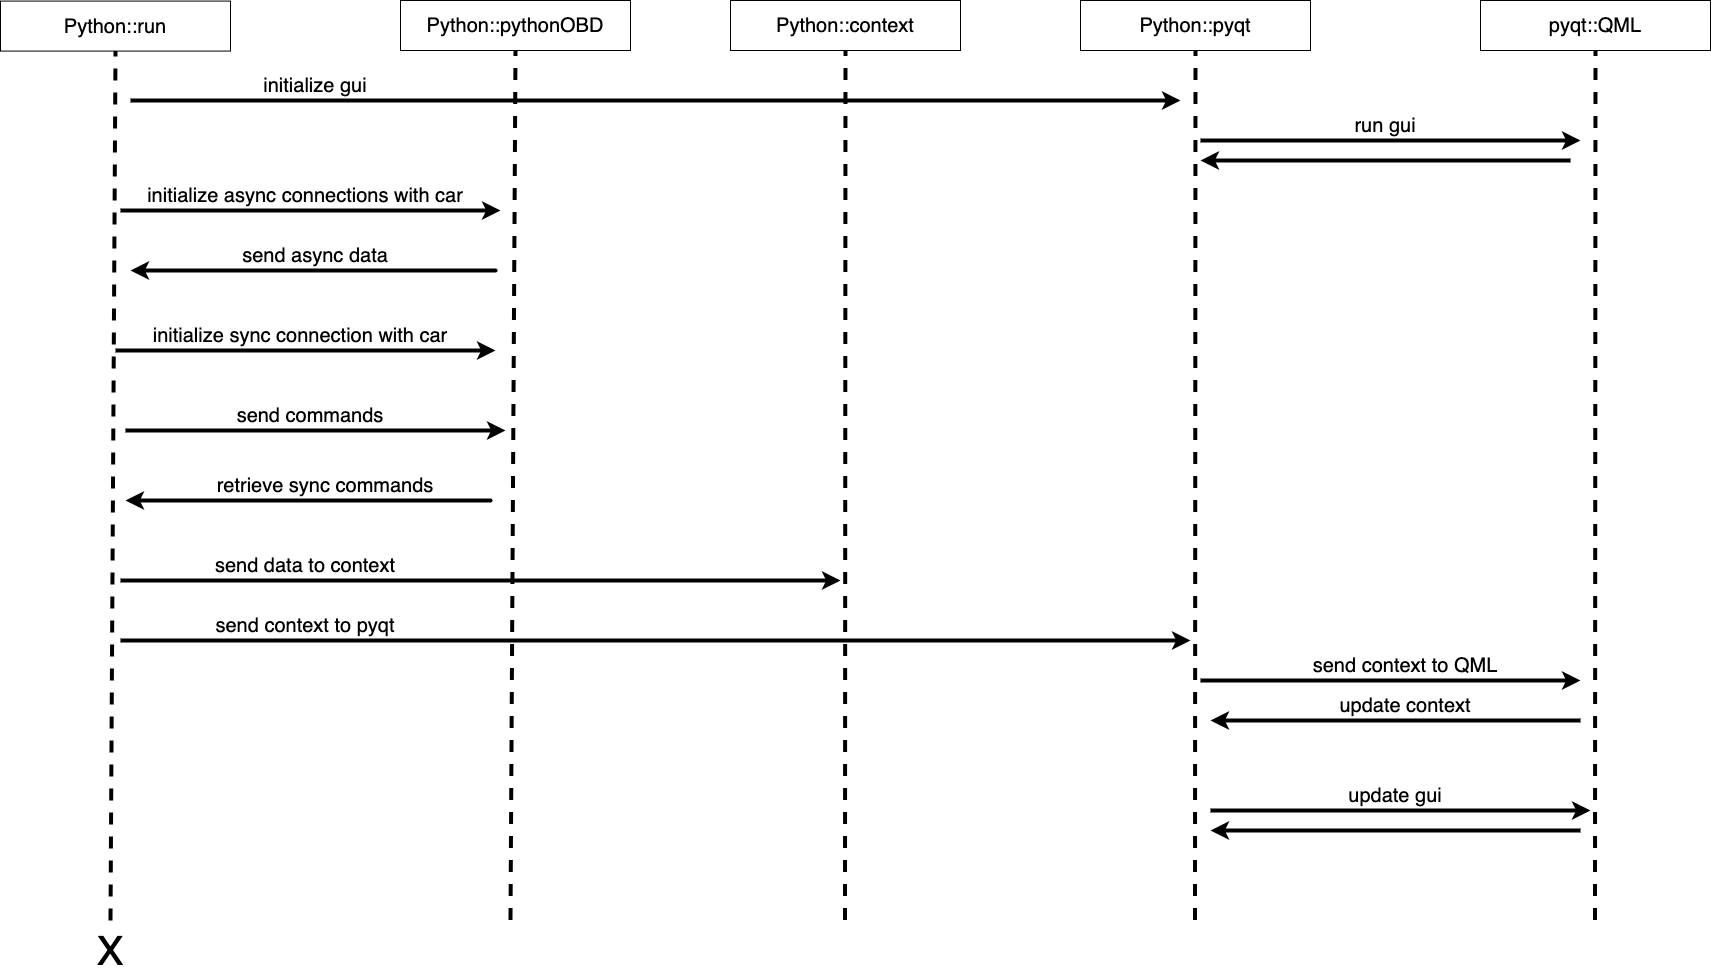
\includegraphics[width=1\columnwidth]{./diagrams/sequence/diagram_sequence.png}
\caption{Sequence Diagram}
\end{figure}





\hypertarget{connecting-the-pieces}{%
\section{Connecting the Pieces}\label{connecting-the-pieces}}

\subsection{Step 1: Gather the Equipment}

\begin{figure}[H]
\centering
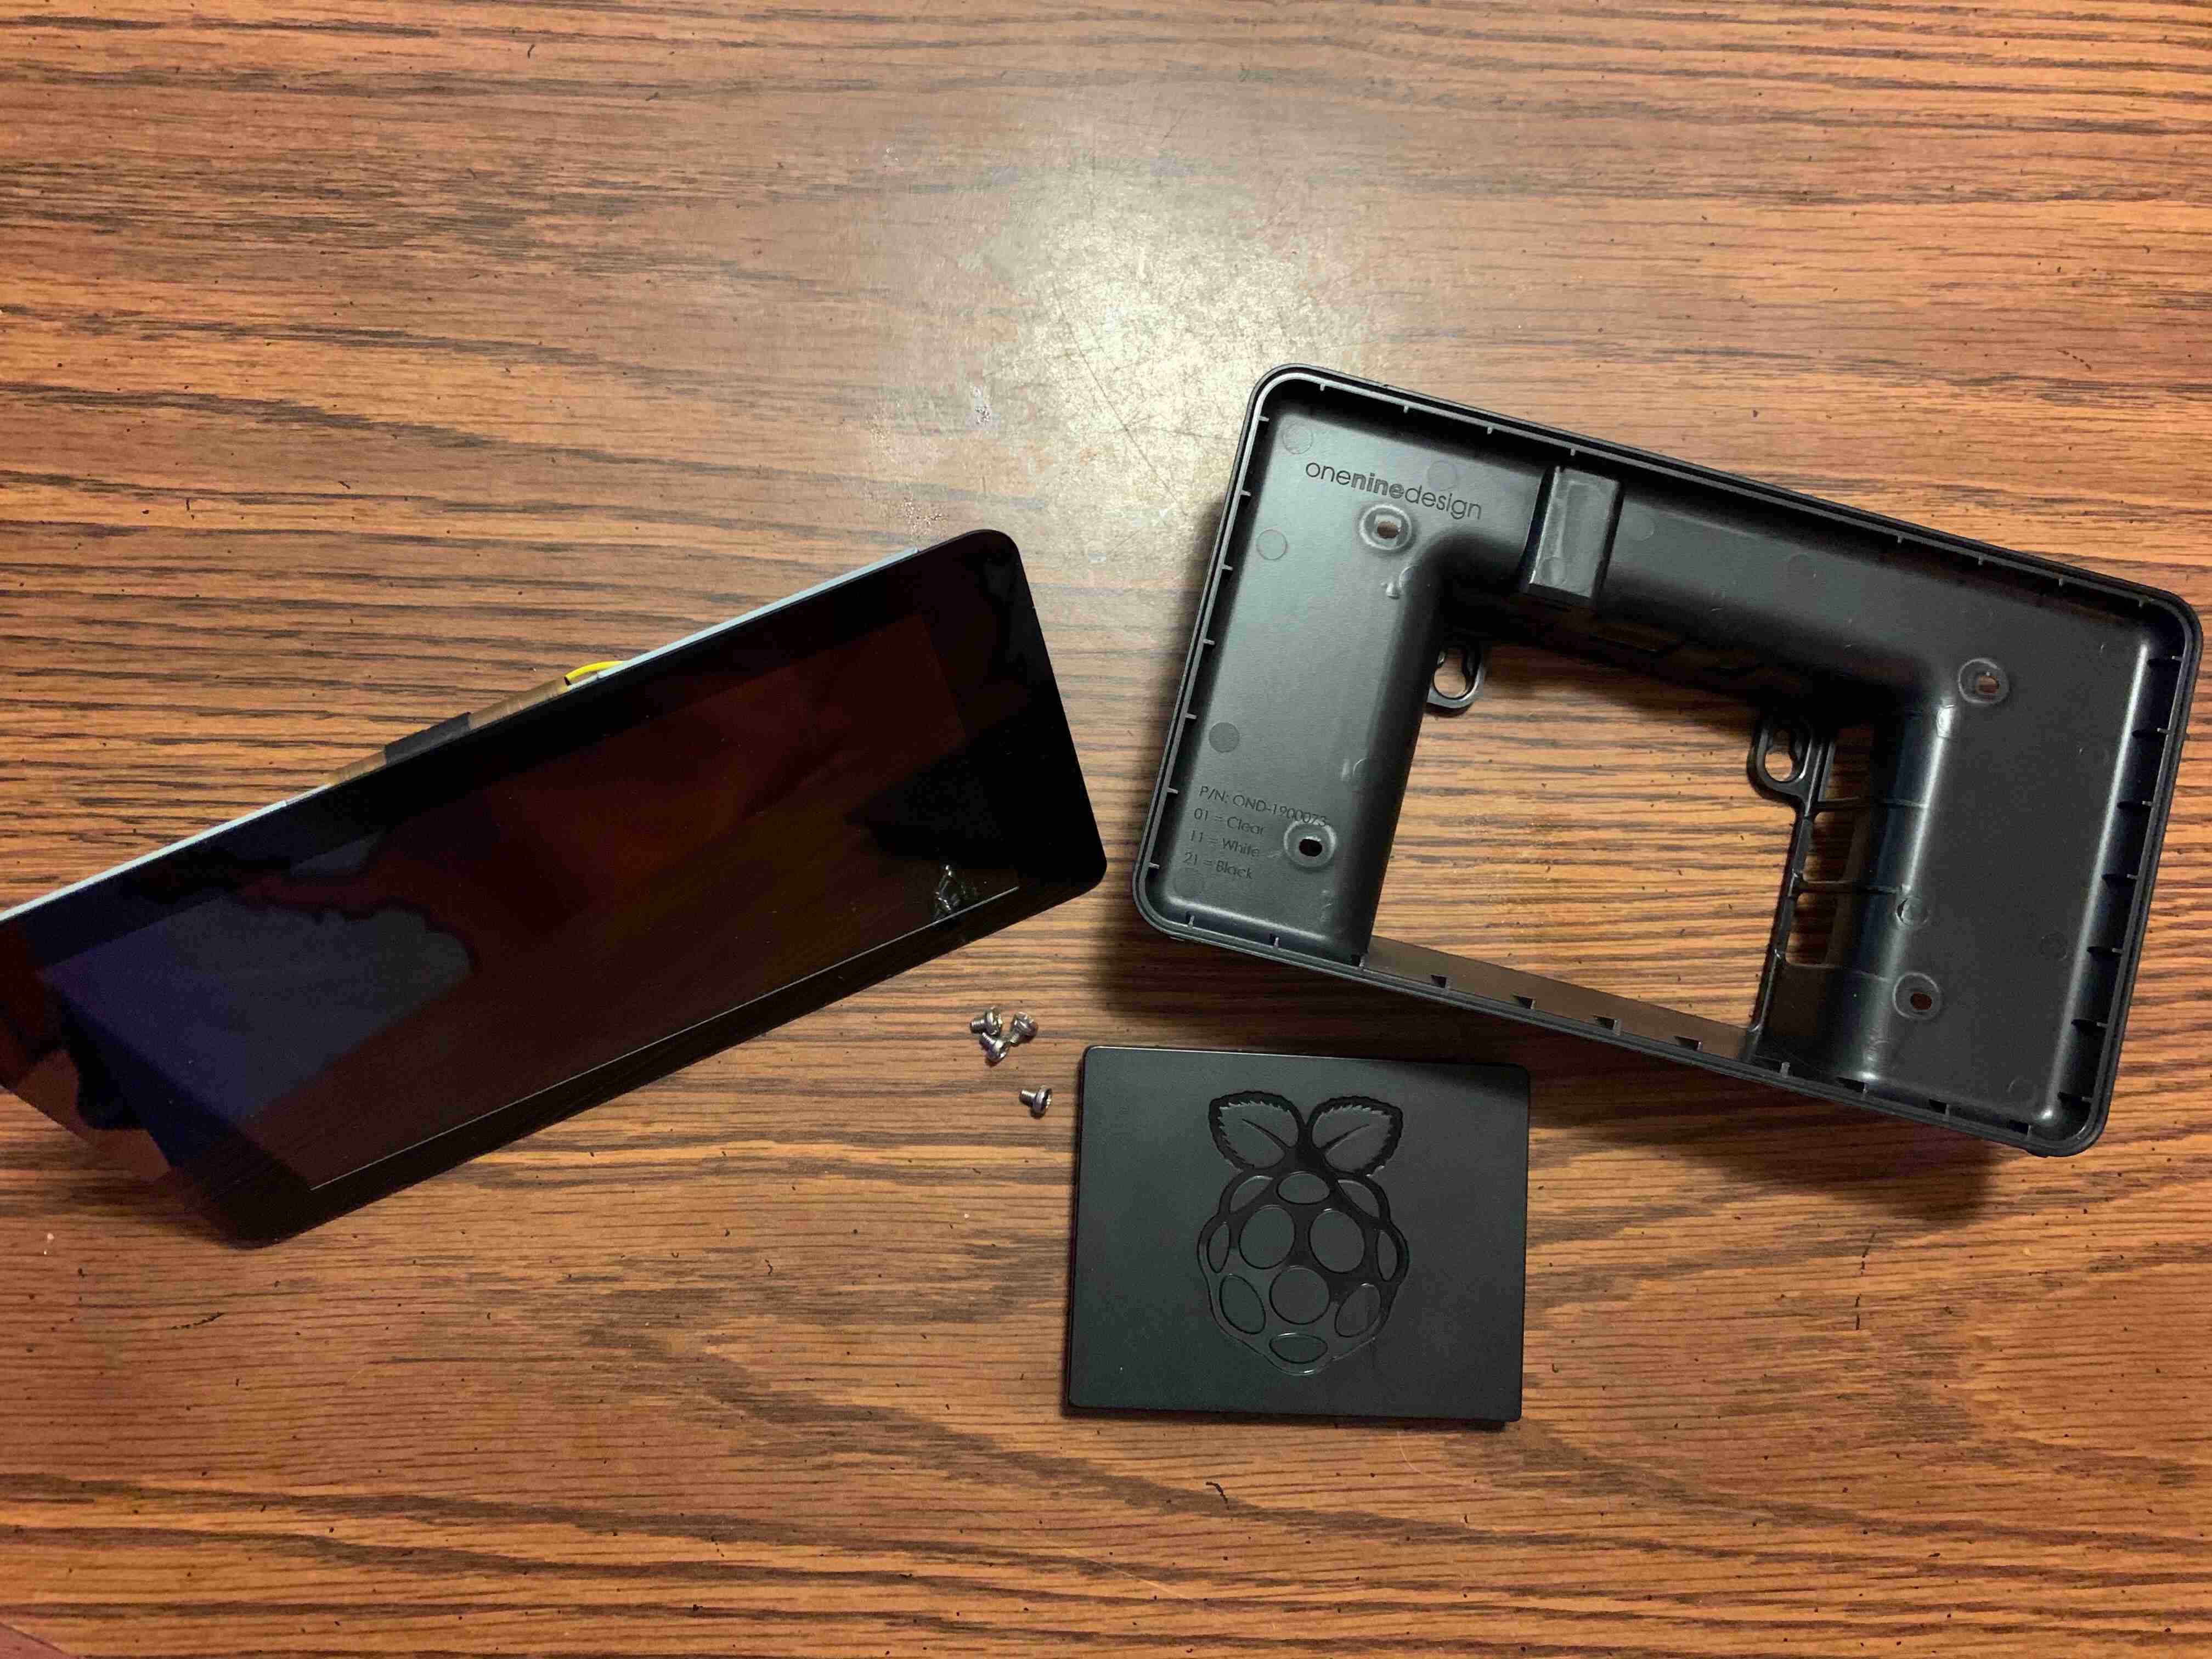
\includegraphics[width=0.7\columnwidth]{./resources/comp-0.jpeg}
\caption{Step 1}
\end{figure}

\subsection{Step 2: Getting Connection}
\begin{itemize}
  \item Screw the raspberry pi into the board posts at the rear of the screen.
  \item Connect the displayport cable from the screen to the Pi (the white ribbon cable)
  \item Connect the pins from the GPIO pins to the screen as pictured in \emph{Figure 4.2}. [pins 1,2 --$>$ pins 1,5]
\end{itemize}

\begin{figure}[H]
\centering
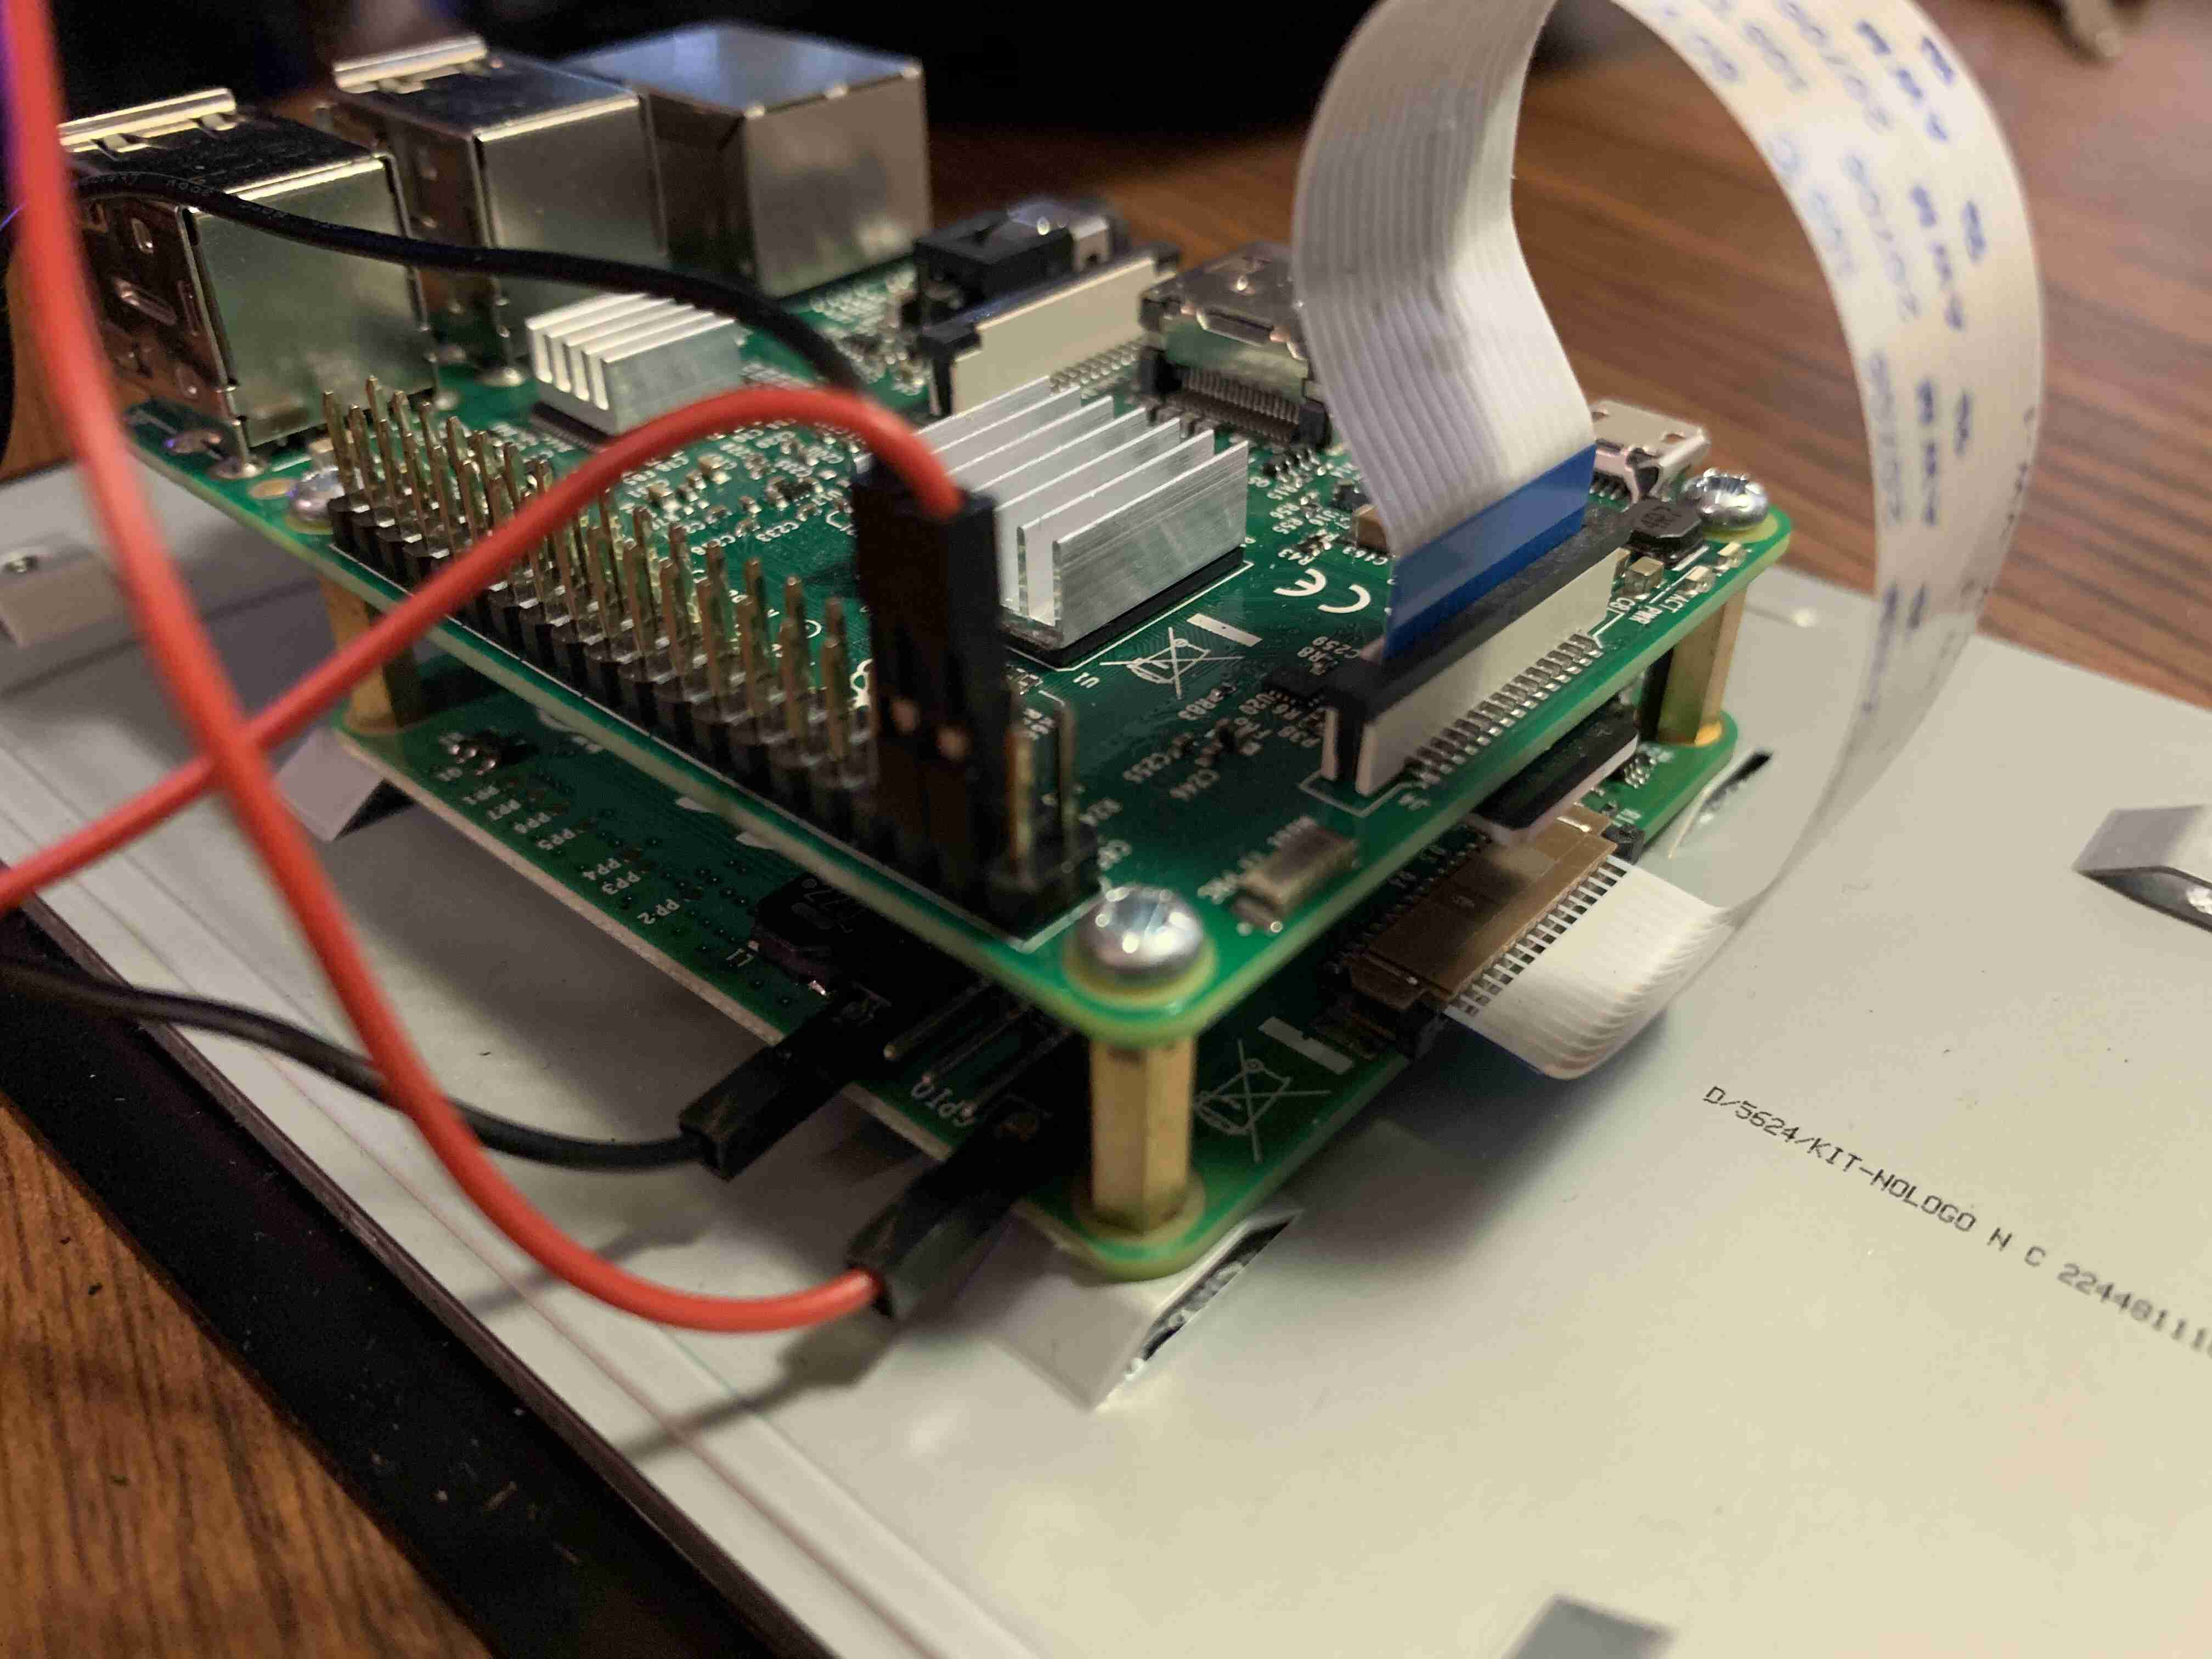
\includegraphics[width=0.7\columnwidth]{./resources/comp-1.jpeg}
\caption{Step 2}
\end{figure}

\subsection{Step 3: RTC Module}
\begin{itemize}
  \item Attach the RTC module to the first four GPIO pins parallel to the previously-connected cables.
\end{itemize}

\begin{figure}[H]
\centering
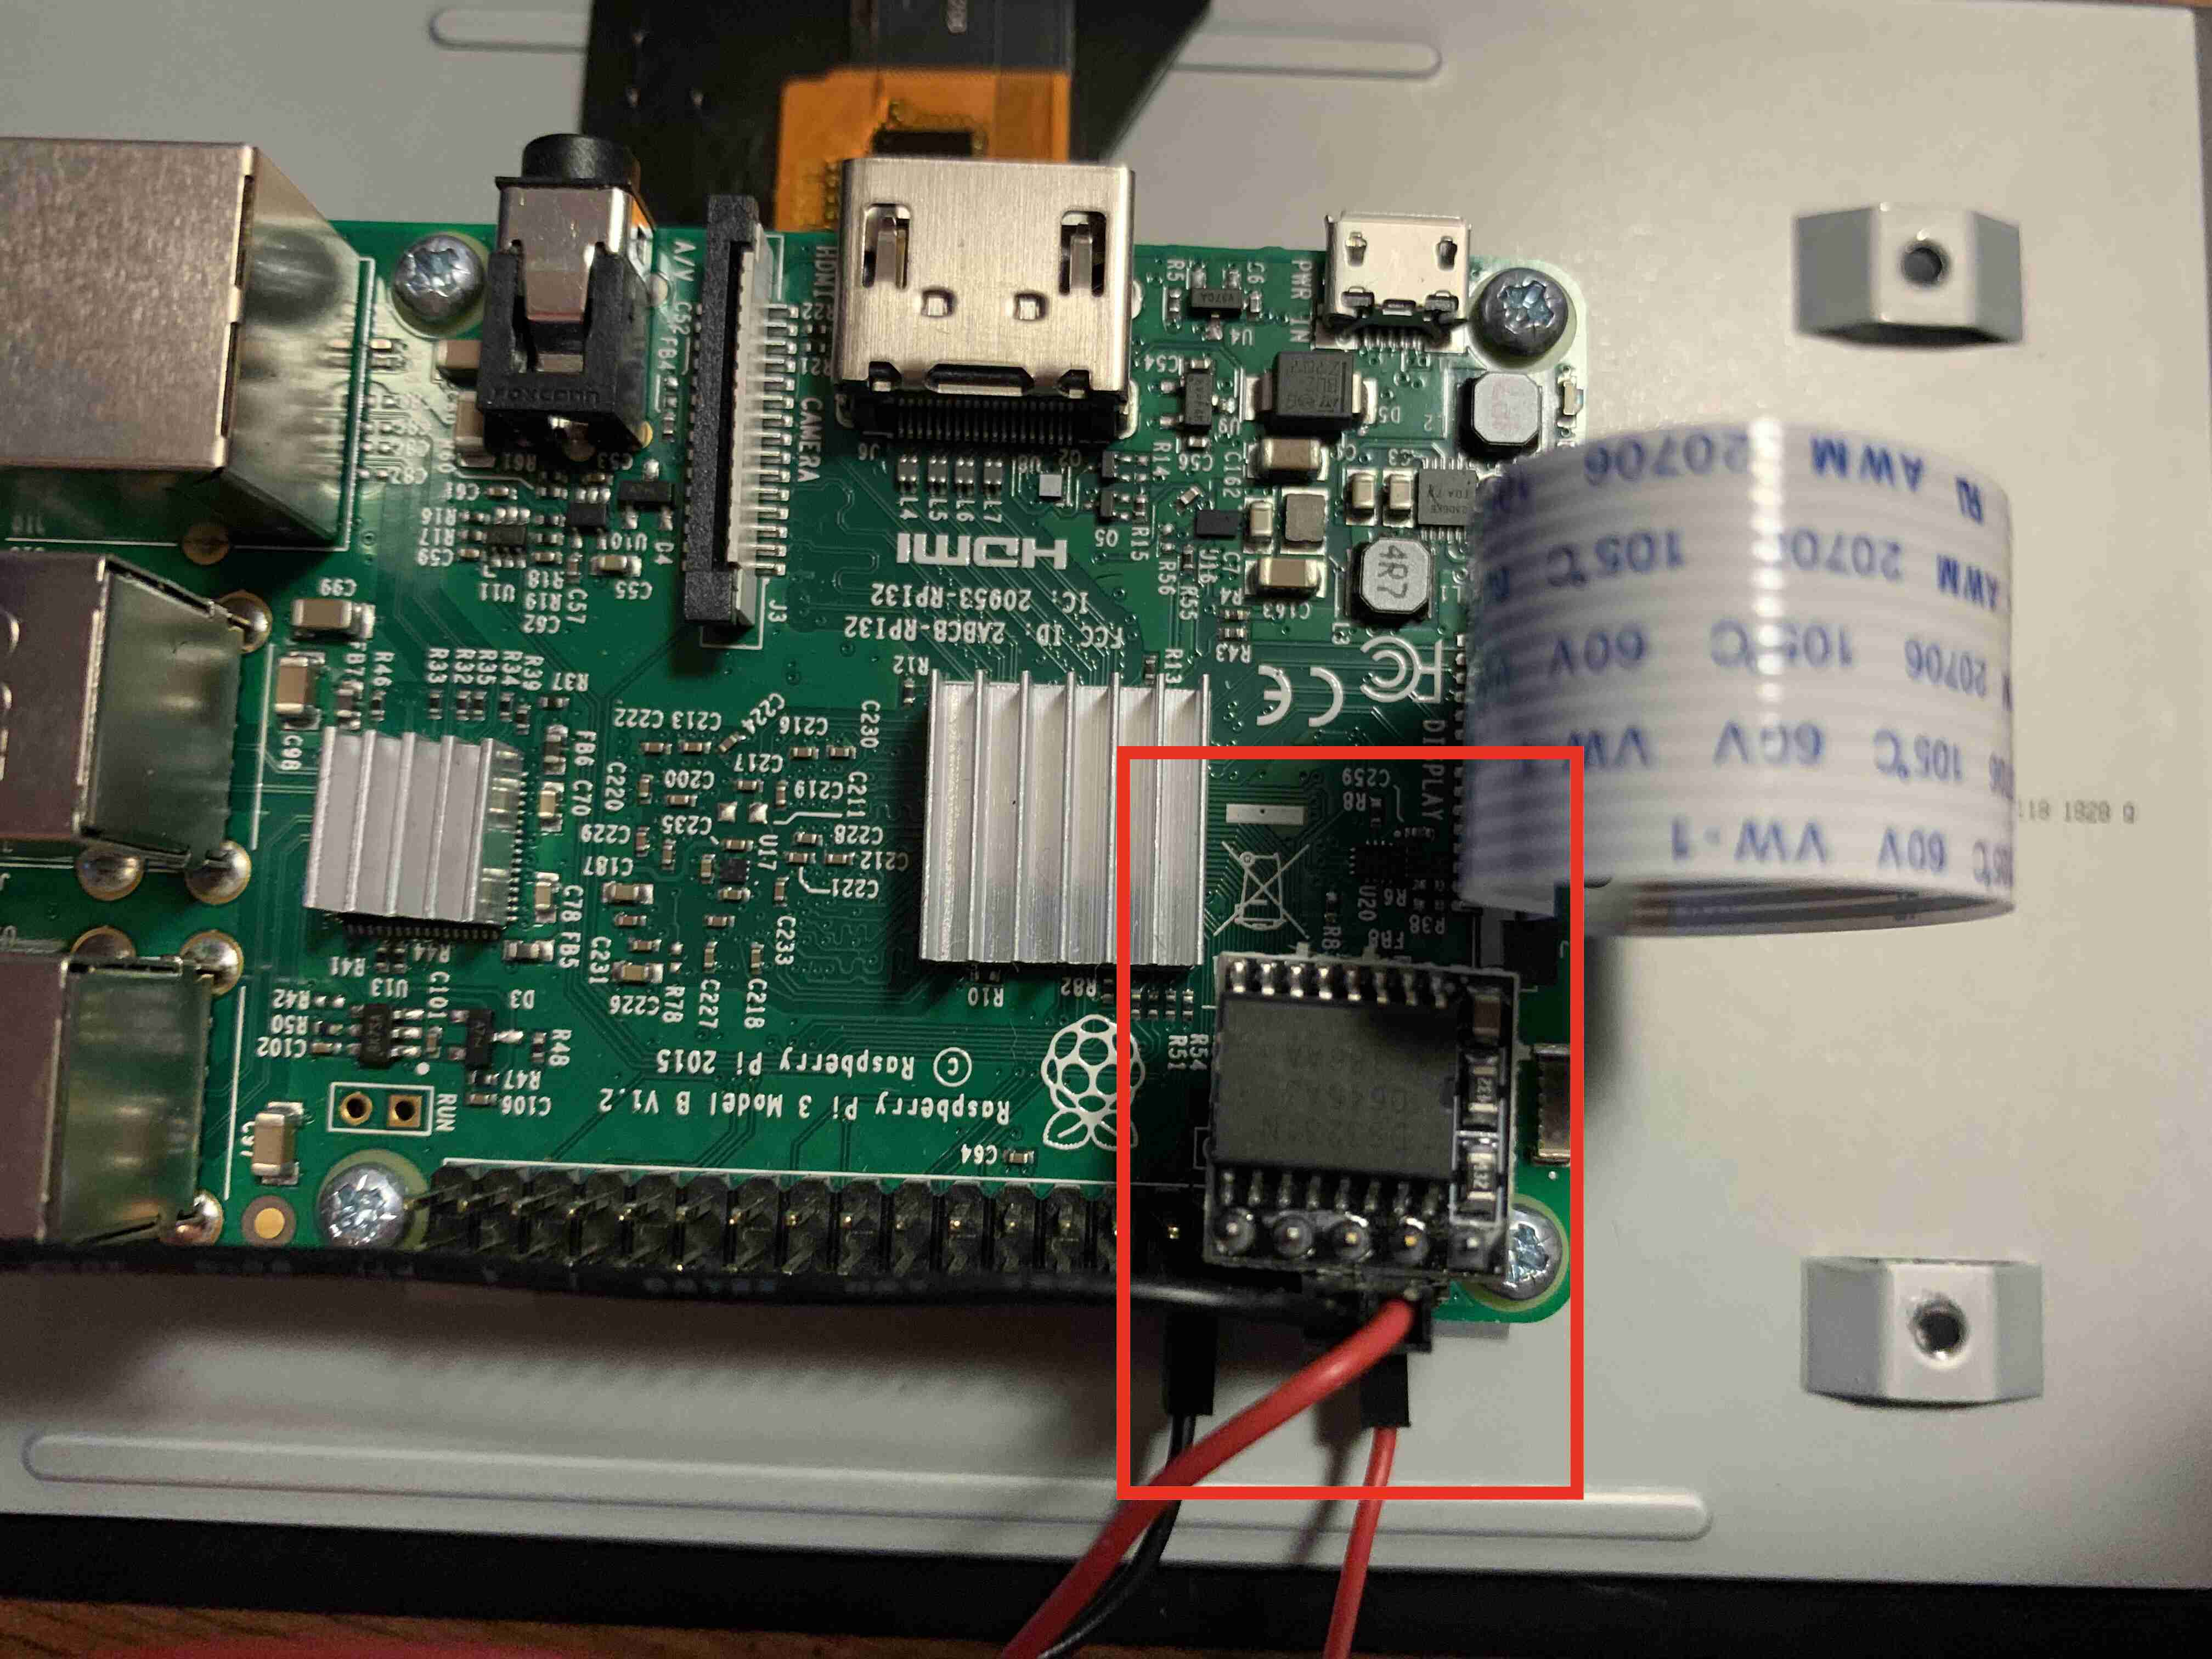
\includegraphics[width=0.7\columnwidth]{./resources/comp-2.jpeg}
\caption{Step 3}
\end{figure}

\subsection{Step 4: Screwing It All Together}
\begin{itemize}
  \item Line up the back casing with the raspberry pi.
  \item Place the screws into each of the four highlighted holes in \emph{Figure 4.4}
  \item Attach the back cover
\end{itemize}

\begin{figure}[H]
\centering
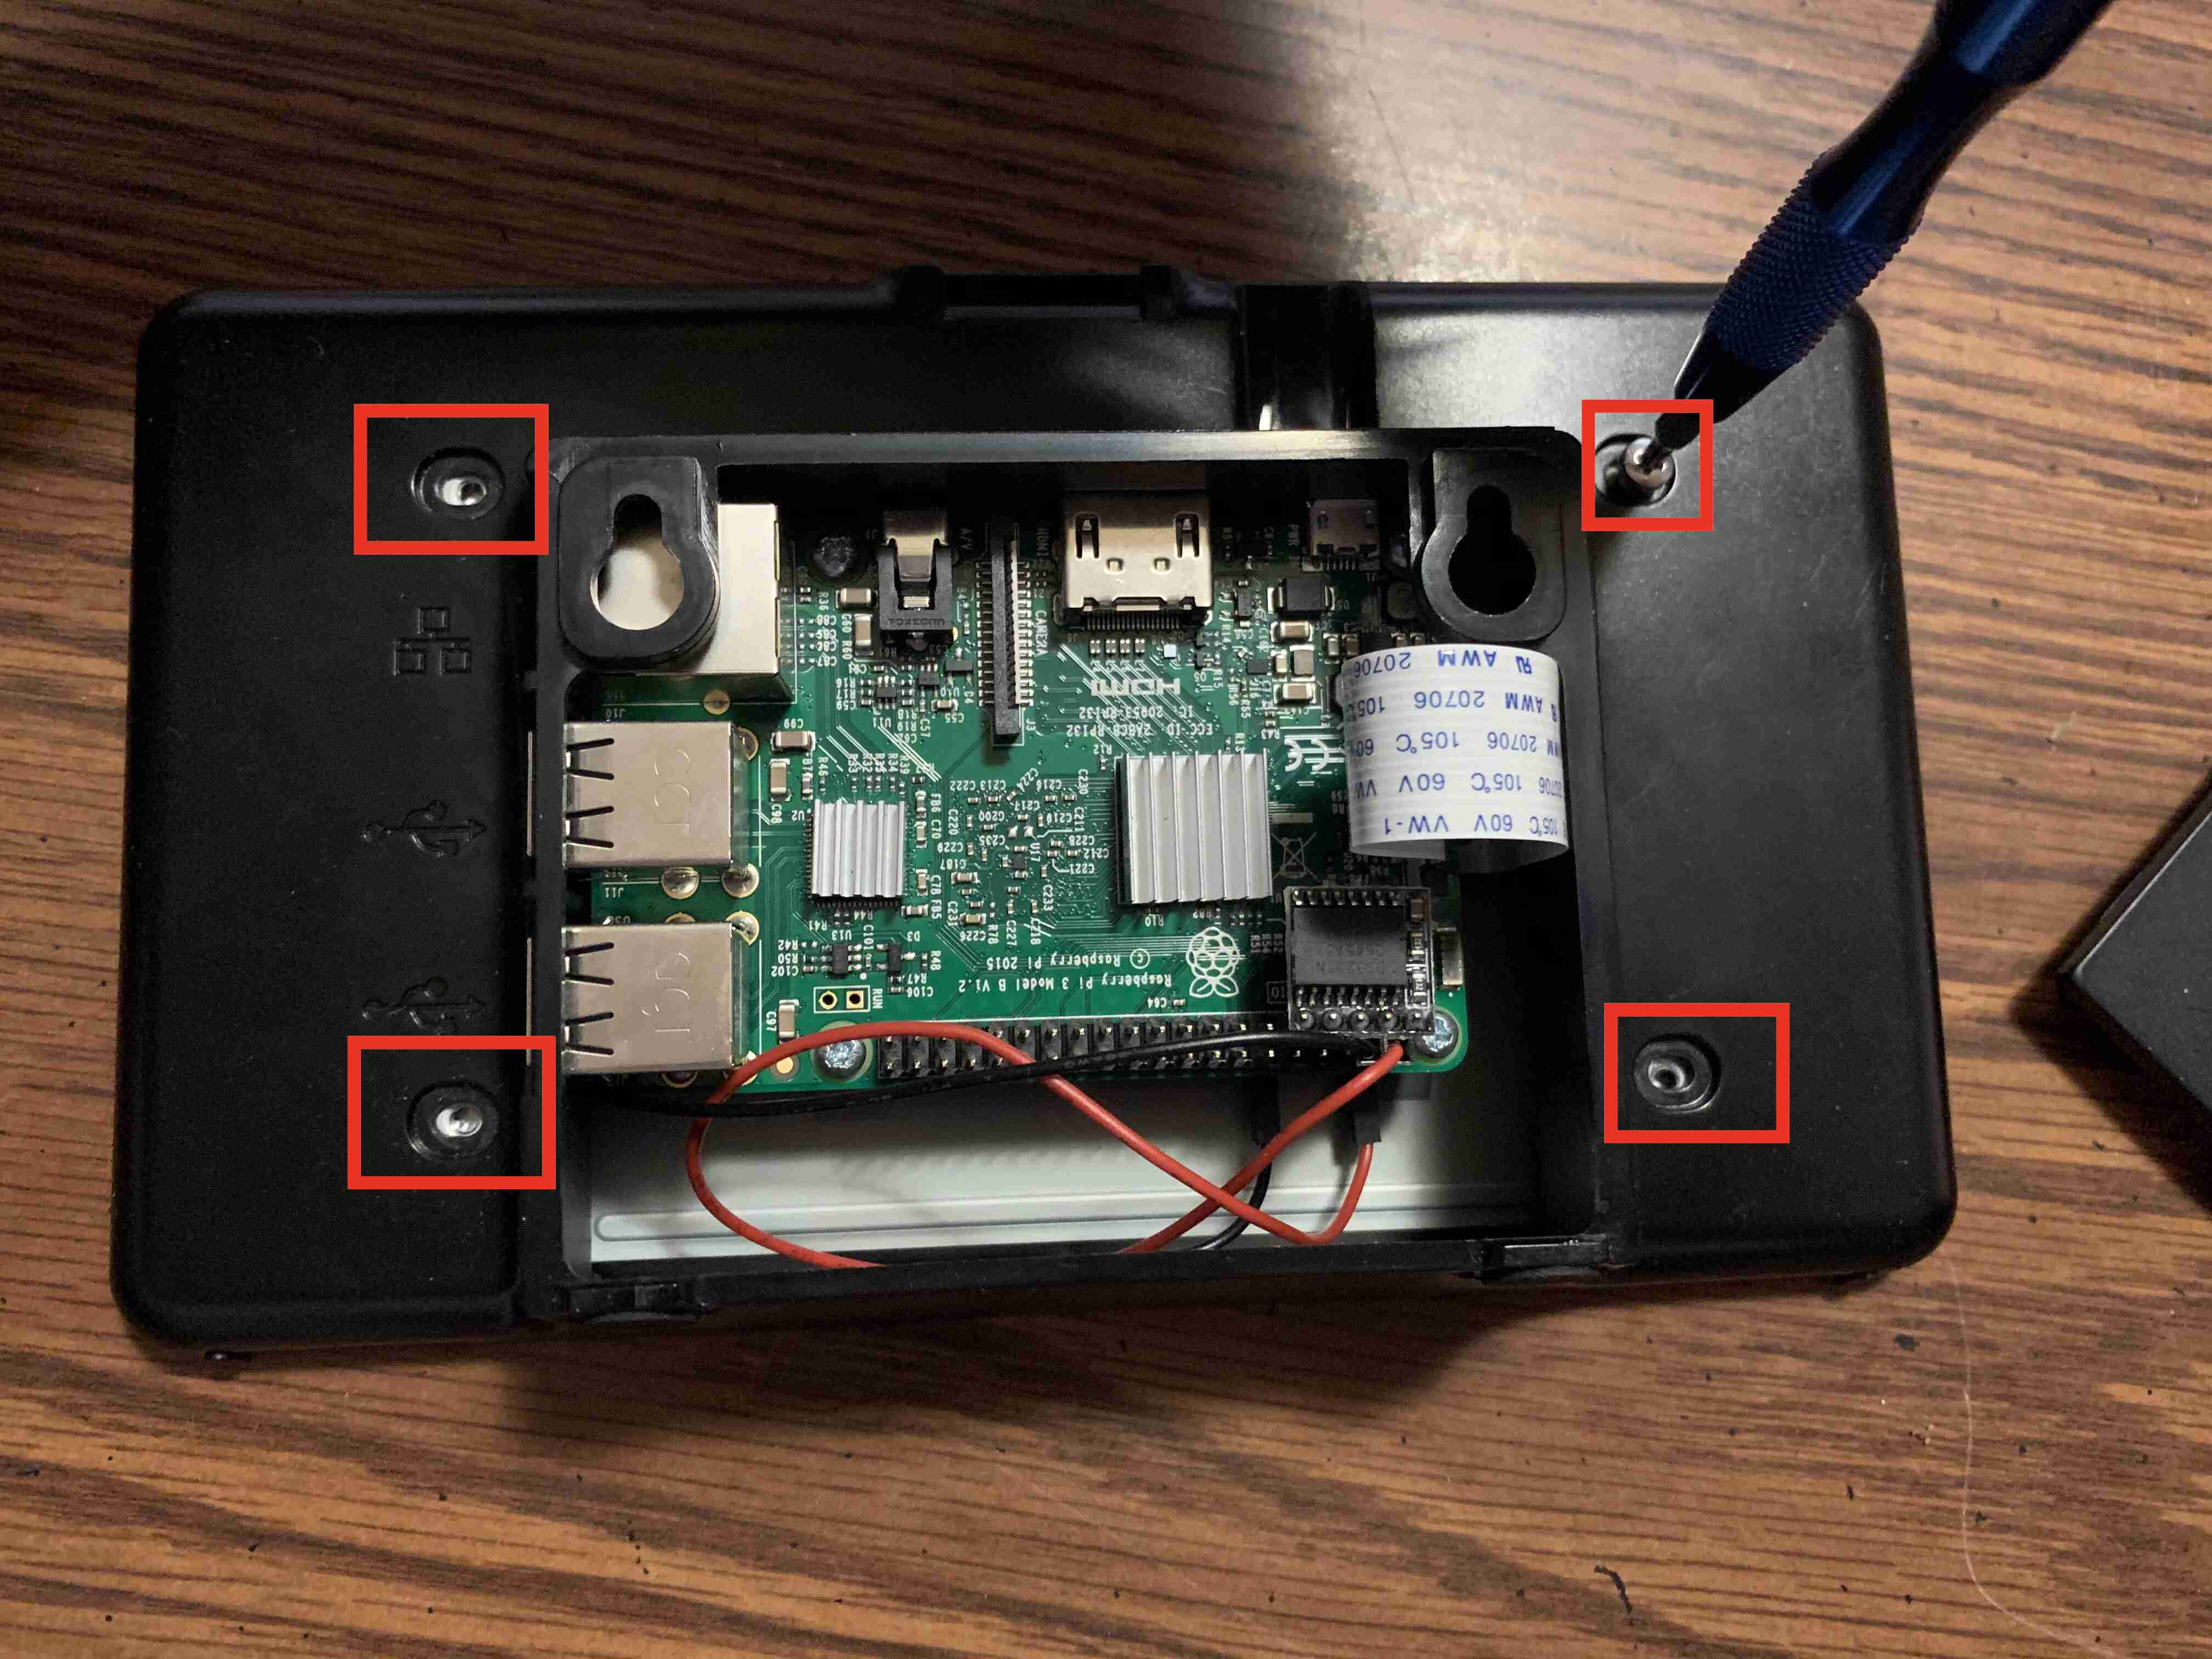
\includegraphics[width=0.7\columnwidth]{./resources/comp-3.jpeg}
\caption{Step 4-1}
\end{figure}

\begin{figure}[H]
\centering
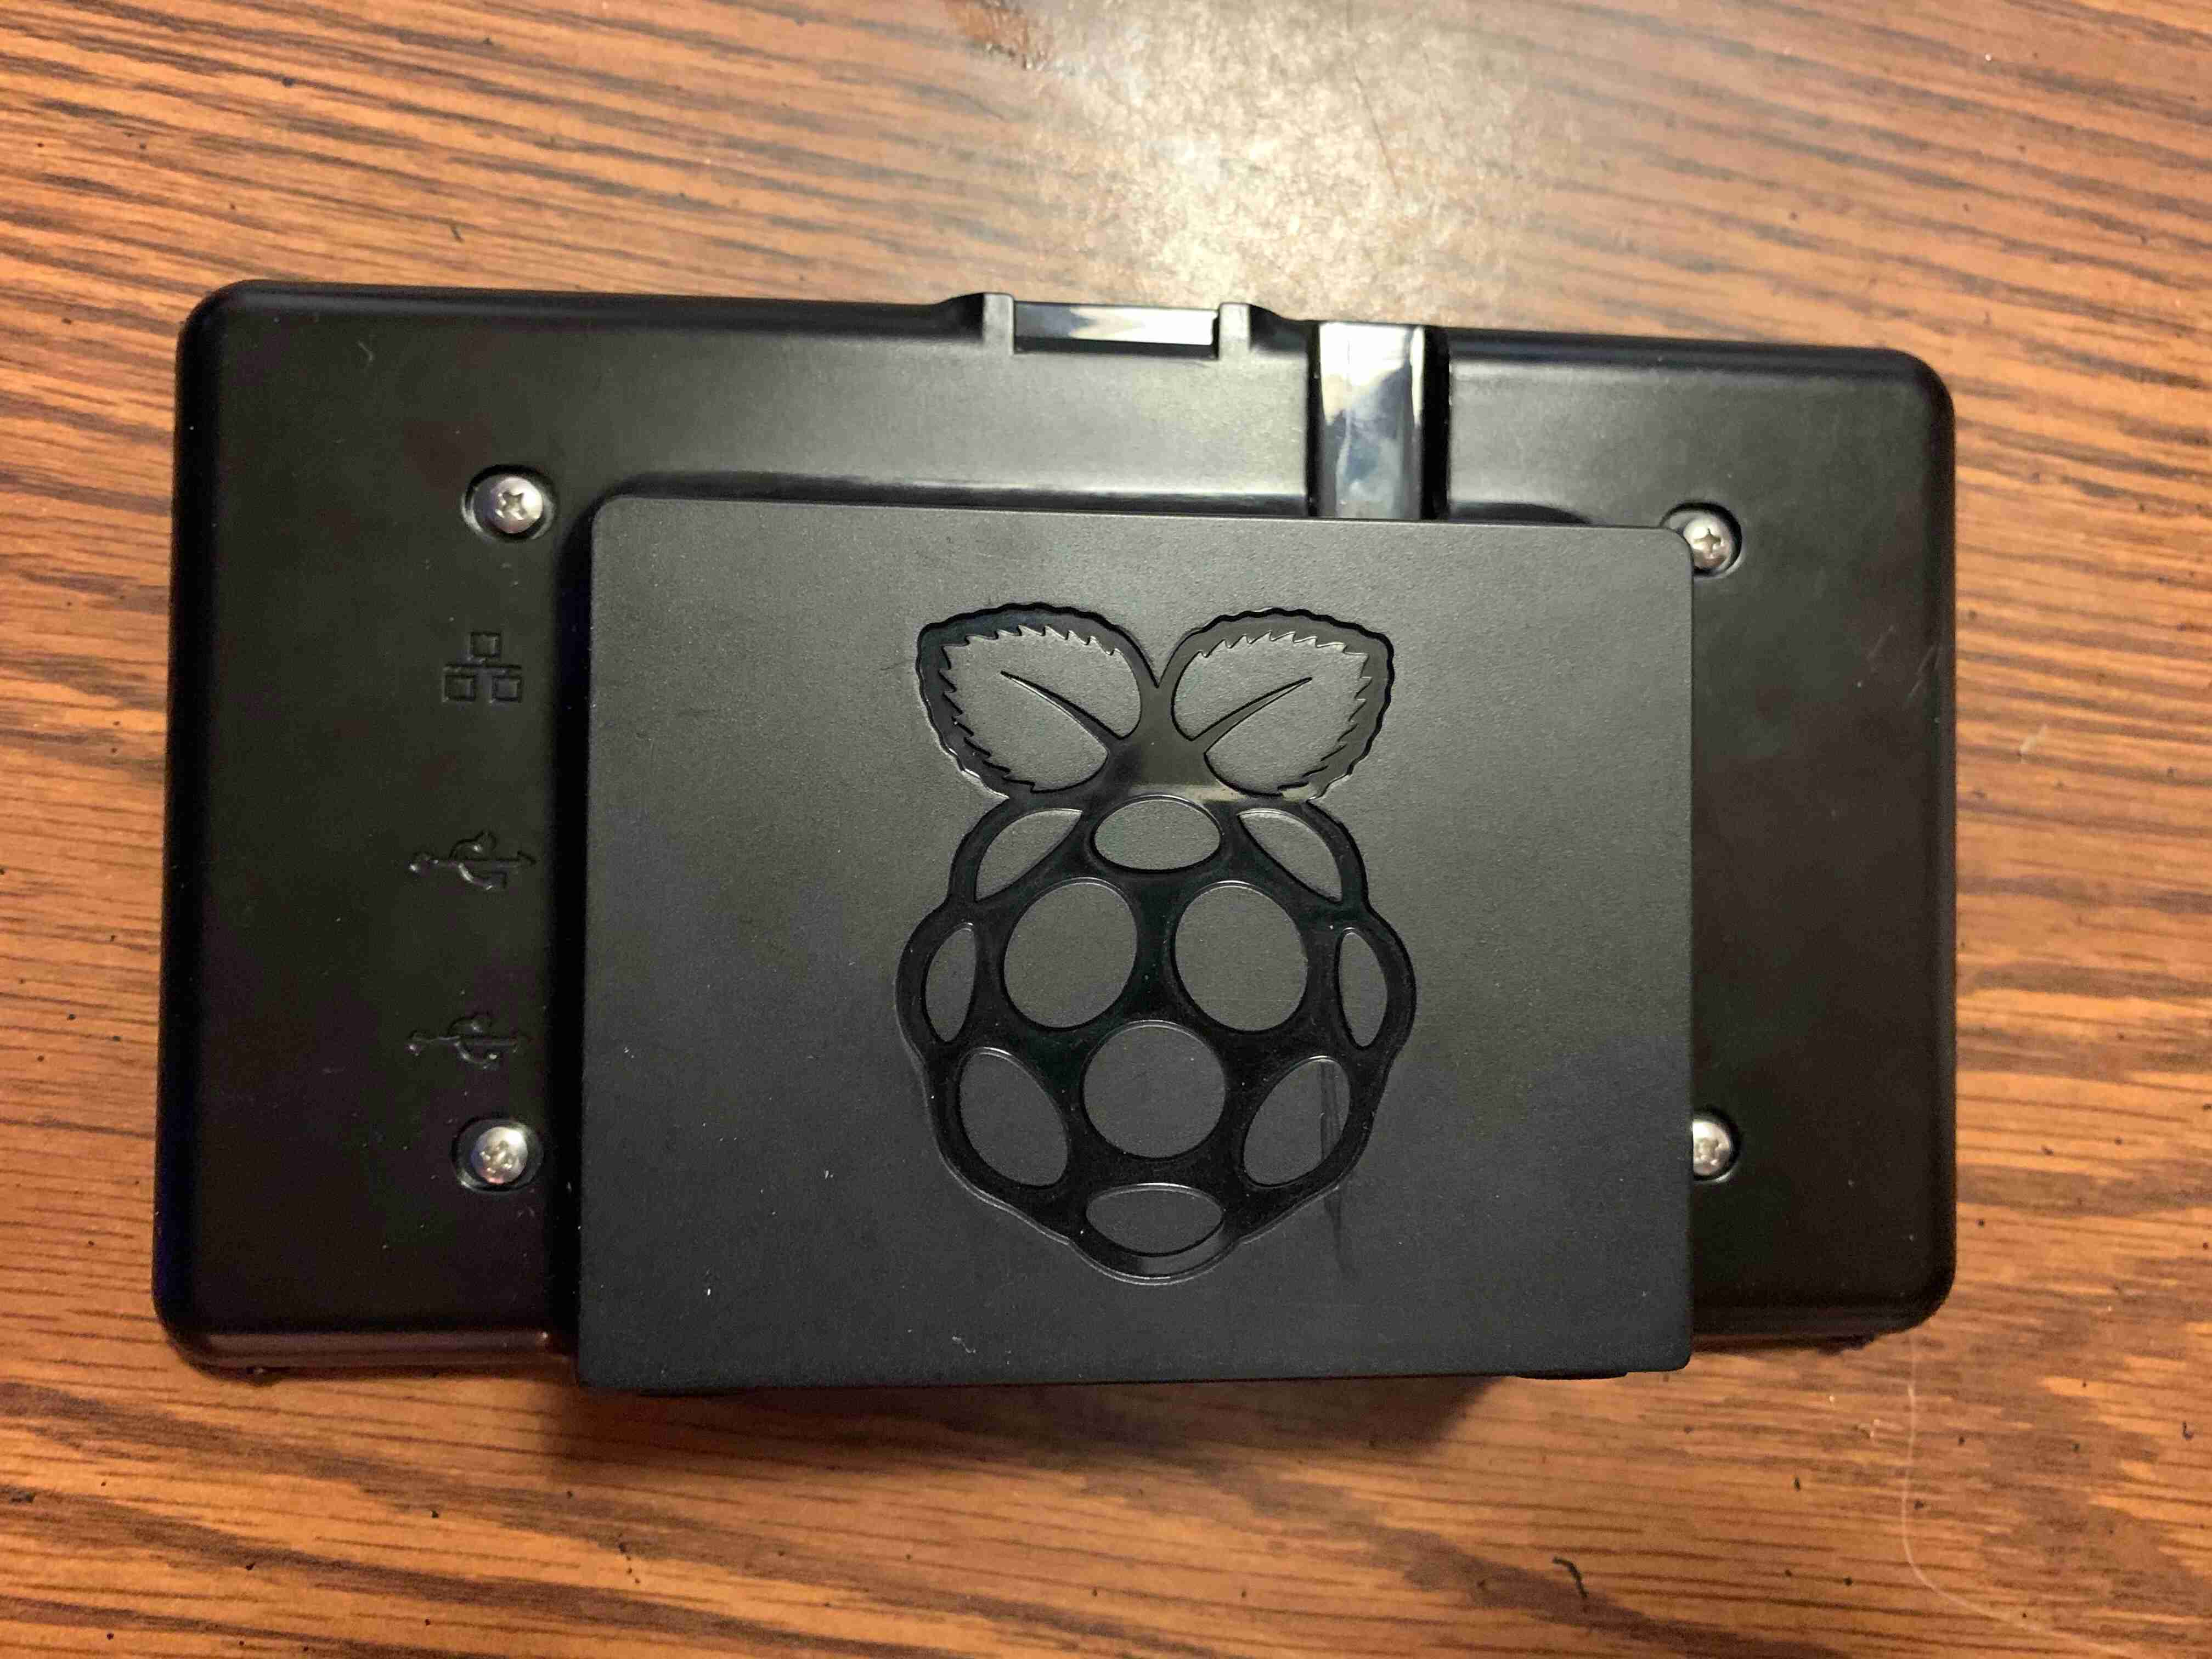
\includegraphics[width=0.7\columnwidth]{./resources/comp-4.jpeg}
\caption{Step 4-2}
\end{figure}

\subsection{Final Product}
\begin{figure}[H]
\centering
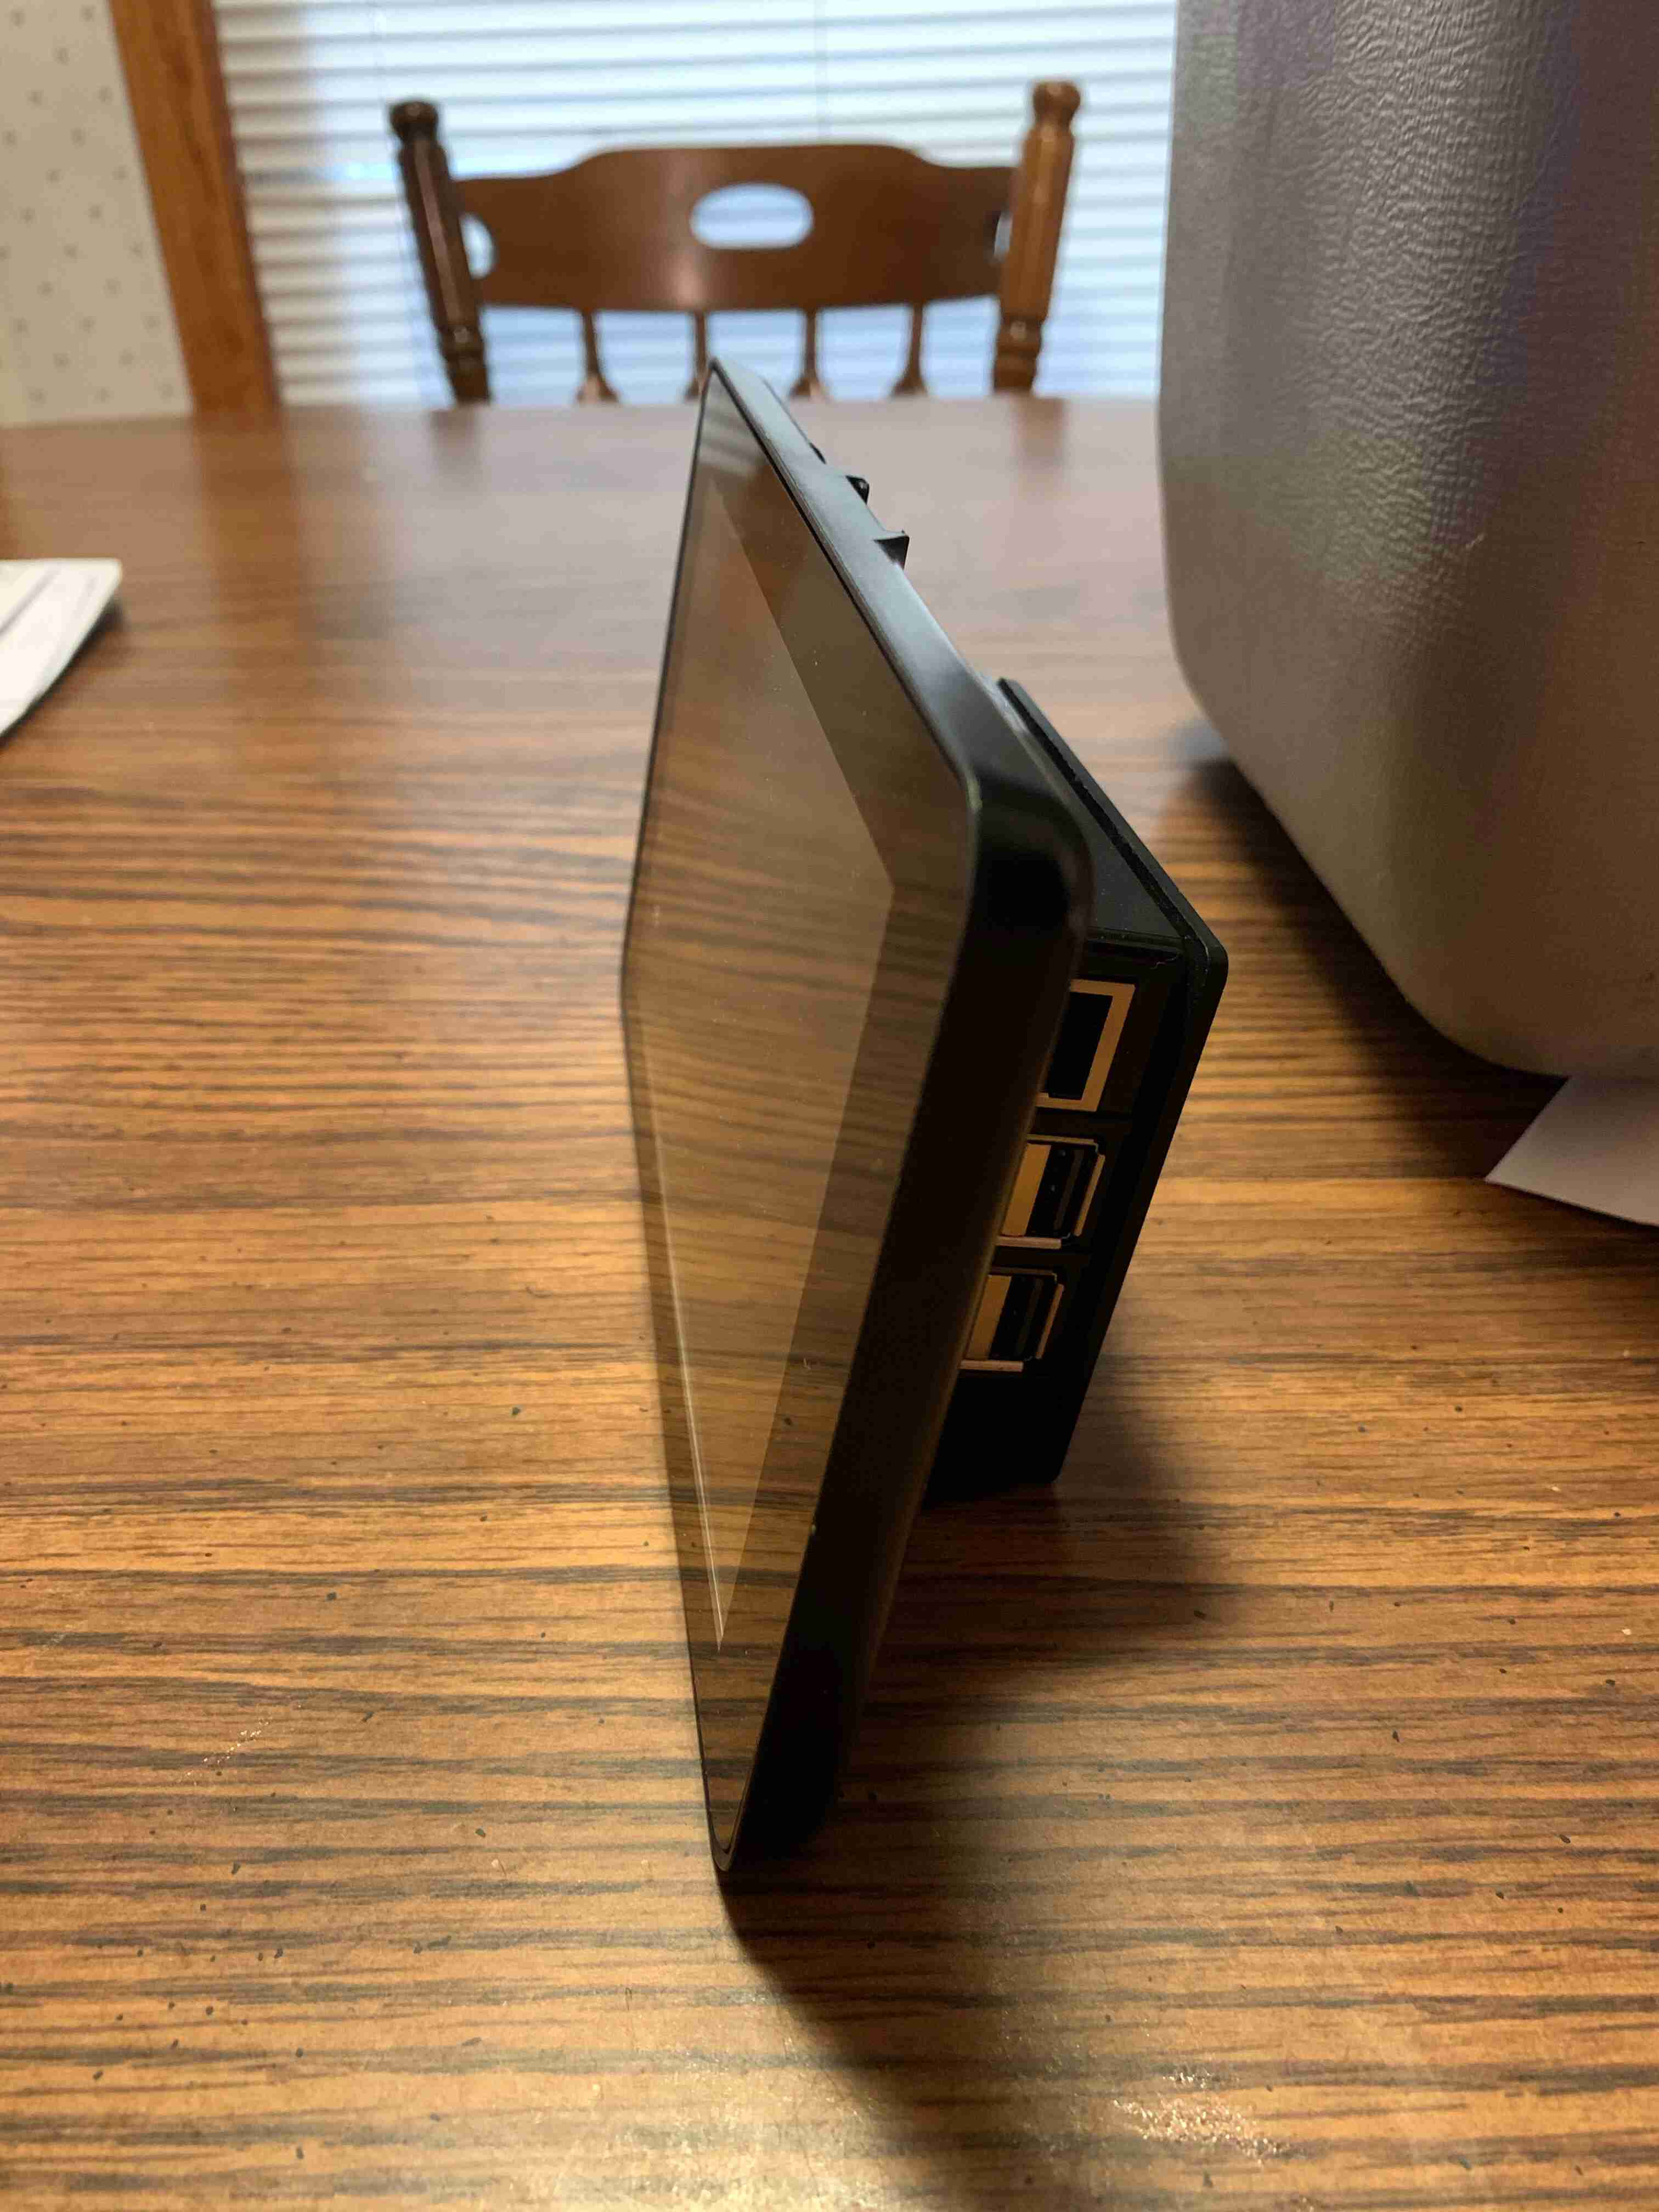
\includegraphics[width=0.5\columnwidth]{./resources/comp-5.jpeg}
\caption{Final Product}
\end{figure}


\hypertarget{getting-up-and-running}{%
\section{Getting Up and Running}\label{getting-up-and-running}}



\hypertarget{recommended-os-dietpi}{%
\paragraph{Recommended OS: DietPi}\label{recommended-os-dietpi}}

The \href{https://dietpi.com}{\emph{DietPi}} (debian-based) operating system distribution acts as a
lightweight desktop environment for running GUIs on the Pi.

\begin{flushleft}
Of Course, you may run this application on another operating system of
your choosing.
\end{flushleft}



\hypertarget{recommended-de-lxde}{%
\paragraph{Recommended DE: LXDE}\label{recommended-de-lxde}}
This project uses \href{https://wiki.lxde.org/en/Main_Page}{\emph{LXDE}}. It is a lightweight desktop environment
that suits the limited hardware of the Raspberry Pi wonderfully.


\paragraph{The use of another desktop environment will require appending a
command that executes the \emph{start\_carberry.sh} script to the
startup file of the respective DE.}

\paragraph{Note: The RTC Module requires the installation of a module-specific driver}

\subsubsection{Installation}
\begin{enumerate}
    \def\labelenumi{\arabic{enumi}.}
    \item   Clone the repo from \url{https://github.com/brohemz/carberry-pi}
    \item   Run \emph{install.sh} in the \emph{/} folder as SuperUser
    \begin{itemize}
        \item Note: The \emph{autostart} functionality of the installation script
                    requires LXDE.
    \end{itemize}
    \item In order to ensure proper \emph{autostart} functionality, restart the computer now.
    \item Run the application \emph{start\_carberry.sh} from \emph{src} folder.
\end{enumerate}
\paragraph{The application should now launch to the main dashboard.}



\end{document}
